% ********************************************
\section{Proposed Framework\label{sec:proposal}}
% *******************************************

We propose an integrated framework for elective surgery planning under uncertainty that links waiting-list management, in-block time management, and operating theatre scheduling. 
Rather than formulating these decisions as a single monolithic model, the framework decomposes the problem into three inter-related modules. 
The first two modules address strategic decisions related to queue and overtime management, and their outputs are then used as inputs to the tactical operating theatre scheduling model. 
Figure~\ref{fig:framework} summarises the proposed framework.

\begin{figure}[htb]
    \centering
    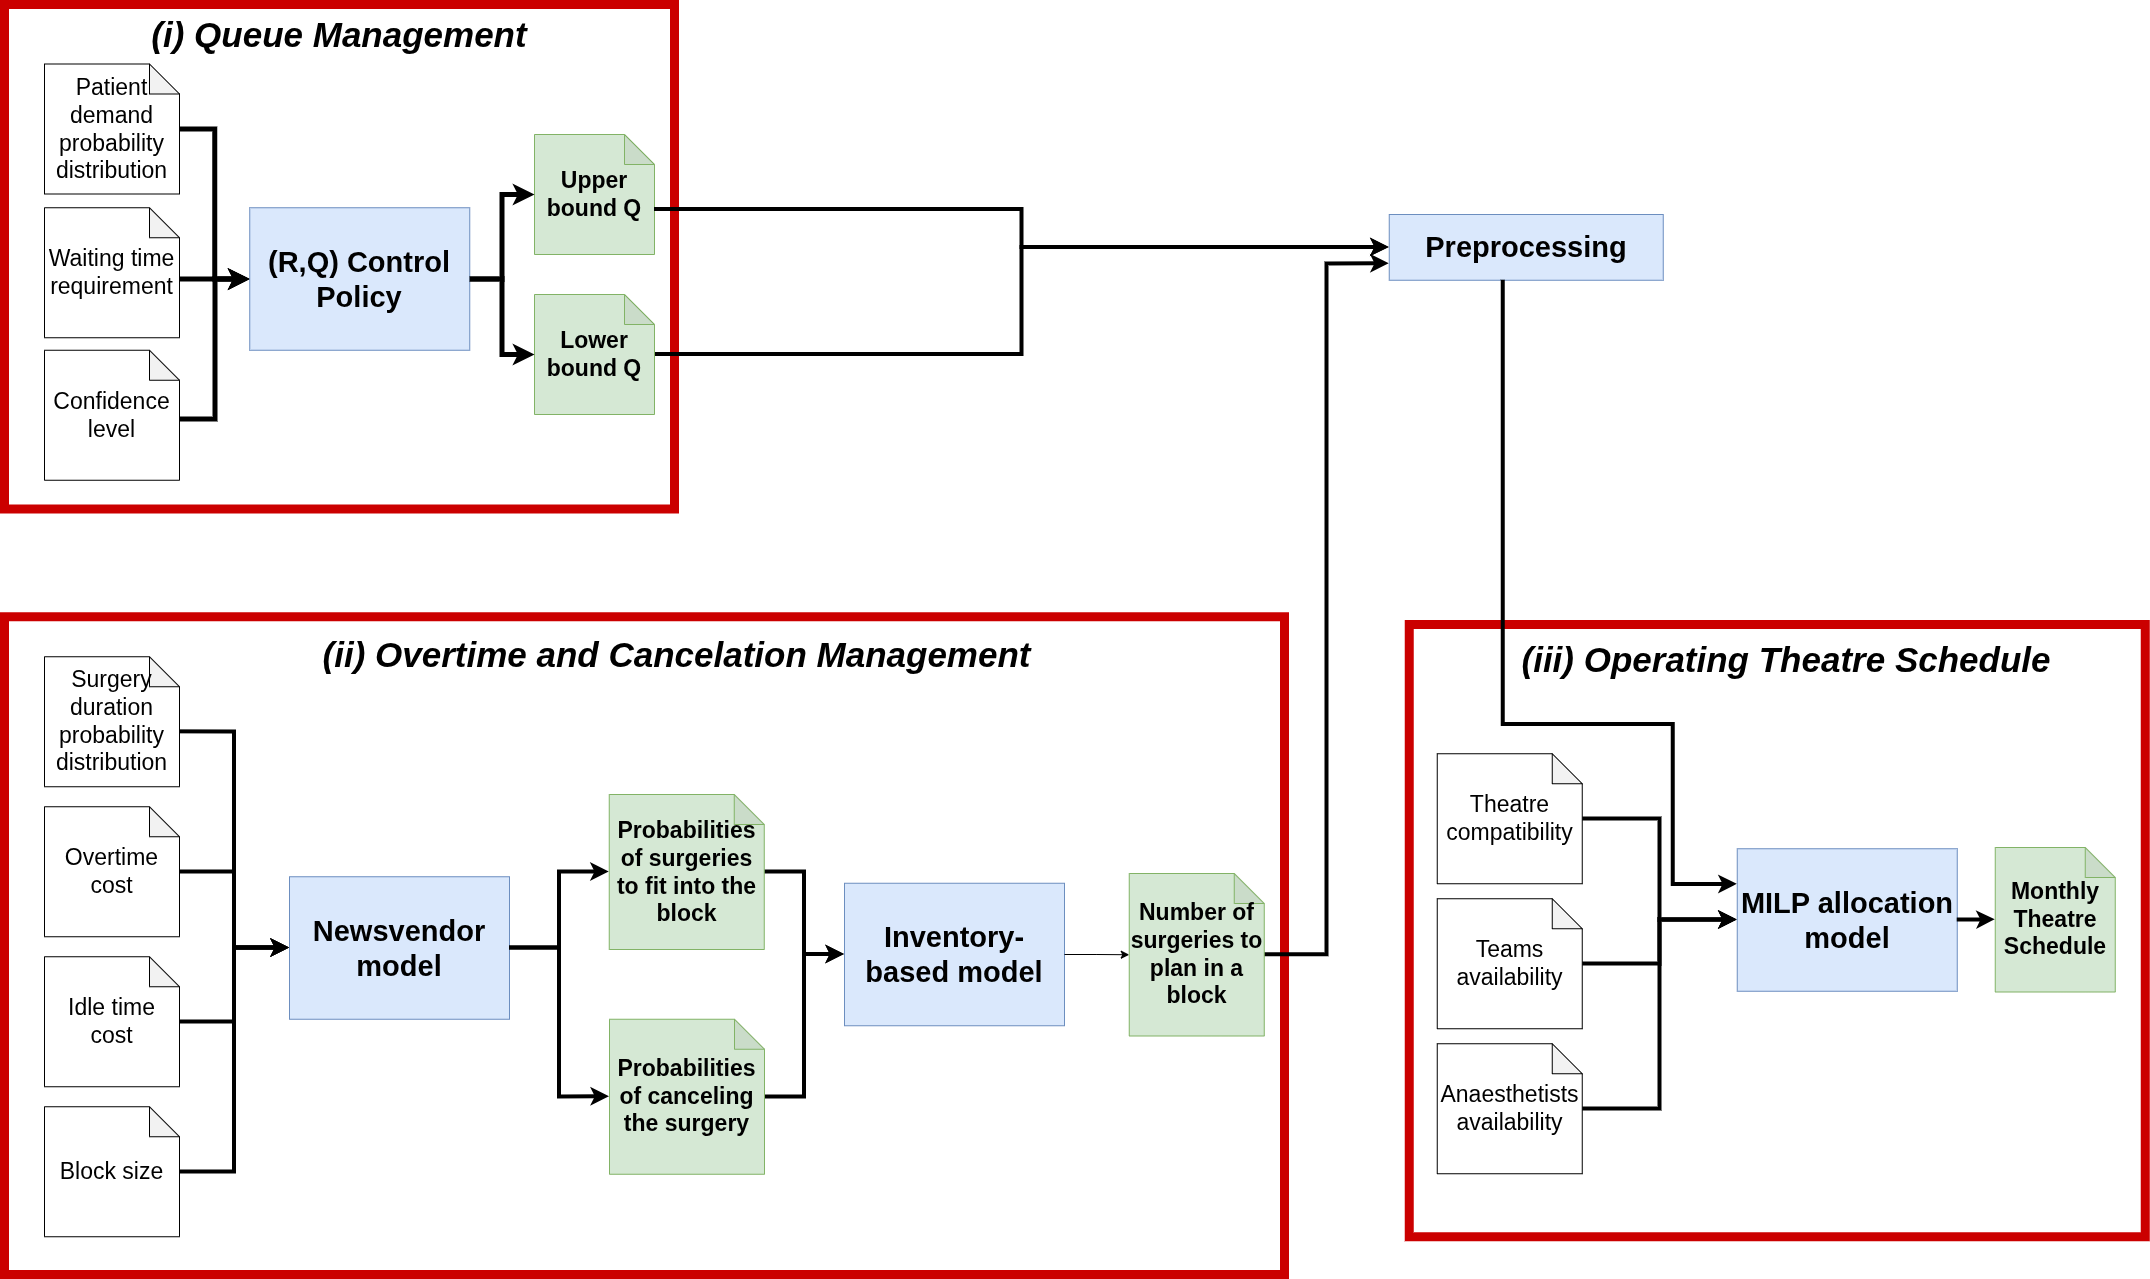
\includegraphics[width=0.9\textwidth]{images/framework.png}
    \caption{Proposed framework.\label{fig:framework}}
\end{figure}

The queue management module establishes targets for the number of surgeries to be performed at each planning period (e.g., monthly). 
Specifically, a modified $(R,Q)$ policy defines, for each medical sub-speciality, a lower and an upper bound on the number of patients to be admitted for surgery during the planning period, while ensuring that system-wide waiting-time requirements are satisfied in spite of the uncertainty in patient arrivals.
% This module supports the long-term balance of the waiting lists by aligning surgery admission with periodic patient arrivals via a classical inventory model under uncertainty.

The second module balances overtime, idle time and the risk of surgery cancellation due to overbooking. Considering the uncertainty in surgery duration, a Newsvendor model guides dynamic decisions on whether to perform or postpone the next surgery, given the time remaining in the session. The output of the Newsvendor model then informs an inventory model that determines the number of surgeries to be booked in a block while balancing the expected number of surgeries with the risk of cancellation.

The outputs of the first two modules are then combined to provide key inputs to the third module, which formulates the OT scheduling problem. 
Specifically, given the probability distribution of the number of performed surgeries per session (module 2), and the bounds on the number of surgeries to be performed in the period (module 1), one can derive lower and upper limits on the number of blocks to be allocated to each surgical sub-speciality. 
Hence, theatre allocation decisions are informed not only by resource availability and clinical compatibility, but also include constraints to guarantee that waiting-time requirements can be met despite the uncertainties in the demand and duration of surgeries. 
Crucially, the scheduling model remains deterministic, thereby facilitating practical implementation and ensuring rapid solution times.

Overall, the proposed framework provides a coherent approach to elective surgery planning across multiple decision levels.  By explicitly incorporating uncertainty into the strategic planning stages, it supports more robust and operationally meaningful scheduling decisions that are guaranteed to align to strategic waiting-time requirements. The following subsections present each module in detail. To help navigate the paper, Table~\ref{tab:acronyms} consolidates the list of acronyms. %For the mathematical notation, we refer the reader to the tables in each module's section.

\begin{table}[htb]
\centering
\caption{Acronyms used in the paper.\label{tab:acronyms}}
\scriptsize
    \begin{tabular}{ll}
        \toprule
        Acronym & Description \\
        \midrule
        CMP & Case Mix Planning \\
        MSS & Master Surgery Scheduling \\
        SCS & Surgical Case Scheduling \\
        OT  & Operating Theatre \\
        MDP & Markov Decision Process \\
        % SAA & Sample Average Approximation \\
        % DRO & Distributionally Robust Optimization \\
        SUS & Brazilian Unified Health System \\
        \hcunicamp & Hospital de Clínicas Unicamp \\
        OTSP & Operating Theatre Scheduling Problem \\
        MILP & Mixed-Integer Linear Programming \\
        PMF & Probability Mass Function \\
        CDF & Cumulative Distribution Function \\
        \bottomrule
    \end{tabular}
\end{table}